\documentclass{thuemp}
\begin{document}

% 标题,作者
\emptitle{不同市场结构下个体动态规划最优解的整体效率
——以车位搜寻为例
}
\empauthor{曹延坤}

% 奇数页页眉 % 请在这里写出第一作者以及论文题目
\fancyhead[CO]{{\footnotesize 曹延坤:不同市场结构下个体动态规划最优解的整体效率 ——以车位搜寻为例}}


%%%%%%%%%%%%%%%%%%%%%%%%%%%%%%%%%%%%%%%%%%%%%%%%%%%%%%%%%%%%%%%%
% 关键词 摘要 首页脚注
%%%%%%%%关键词
\Keyword{市场结构;结构设计;动态规划;搜寻匹配;社会效率}
\twocolumn[
\begin{@twocolumnfalse}
\maketitle

%%%%%%%%摘要
\begin{empAbstract}
本研究从真实现象切入,以自行车停车问题为出发点,揭示了其作为搜寻匹配和动态决策问题的本质;并从自行车停车场的空间设计对车位利用率的影响推广到市场结构和制度设计对资源使用效率的影响上。本文认为在鼓励行为主体进行创新、探索等风险性行为时,仅仅通过提高其期望收益、给予前期保障是难以达到资源充分利用的;还必须为行为主体提供良好且可得的备选项。
\end{empAbstract}

%%%%%%%%首页角注,依次为实验时间、报告时间、学号、email
\empfirstfoot{2022012457}{cyk22@mails.tsinghua.edu.cn}
\end{@twocolumnfalse}
]

%%%%%%%%!首页角注可能与正文重叠,请通过调整正文中第一页的\enlargethispage{-3.3cm}位置手动校准正文底部位置:
%%%%%%%%%%%%%%%%%%%%%%%%%%%%%%%%%%%%%%%%%%%%%%%%%%%%%%%%%%%%%%%%
%  正文由此开始
\wuhao 
\enlargethispage{-0.5cm}

\section{引言}
\par 关于福利保障是否应该存在,经济学界有着不同的看法。当人们已经位于良好的处境时,有的人会因为感到安全且有保障而更愿意去冒险;有的人则会因为感到满足而不愿意去冒险。本文认为,决定人们是否更愿意去冒险的因素不仅是事前已有的处境,而且与事后的备选项有关。
\par 例如在清华大学某办公楼门口曾有一现象:唯一的办公楼大门位于自行车可通行道路的尽头,即自行车只能从一个方向前往大门。但此时自行车停车的聚集处并不集中在最靠近大门的地方,而是略靠近大门但离大门仍有一小段距离的位置;不仅如此,此时最靠近大门的地方甚至仍有空余车位。师生不愿意继续向前寻找车位可以被理解为其找不到车位并返回的期望效用损失与找到车位的期望效用增益相等。不同的是,在学校南区学生宿舍楼下,宿舍楼唯一的入口大门位于道路的中间,即自行车可以从两个方向前往目的地,这导致最靠近入口大门的地方车位基本上总是被占满的。这可以理解为,当学生们在一侧找不到车位时,可以前往另一侧继续寻找,因此不用折返回到上一个找到的车位。
\par 由此可以推测在动态搜寻的过程中,即使在起始点相同、效用函数相同的情况下,不同的停车场结构也会对个体决策产生不同影响,并导致最后整体资源利用率存在差异。所以本文意图使用数学模型证明并推广这一点,从而为提高公共资源利用效率提供有益理论支撑。
\par 当前学界对类似问题的研究大多以“停车者”为中心,关注其在不同“停车场”结构下的最优搜寻策略。例如\citet*{krapivsky_simpleparkingstrategies_2019}比较了在单向通道停车场中停车者的三种策略,分别是“保守(Meek)”,“谨慎(Prudent)”和“乐观(Optimistic)”,并发现在大多数情况下,谨慎策略的表现最优。但是这三种策略均缺乏动态决策机制,而本文模型中停车者统一采取的策略,在期望效用的基础上包含了动态决策以及停车者对空车位概率分布的估计。这种策略最接近“谨慎策略”,但与其显著不同。
\par 本文不仅在搜寻策略上有所改良,而且着重强调“停车场”的整体效率,即市场本身应该如何规划整体结构以使得其中最优的“车位”被充分利用,这一问题被当前大部分研究所忽略。当前关注到市场结构的研究对市场结构的理解较为多样,主要关注市场竞争结构和企业决策\citep*{bar-isaac_searchdesignmarket_2012, DuChuang_pingtaineishichangjiegoushejijianlunwangshangwaimaishangyemoshiyuguanzhi_2024}、市场主体集体行为的经济后果\citep{becker_irrationalbehavioreconomic_1962}、市场不同垄断水平的效率差异\citep{MengShanShan_shichangjiegouchuangxinshouyigongyinglianfenpeiyuchanyefazhan_2024a}等。少数从市场机制上考察市场结构的研究主要以拍卖形式为落脚点\citep{lucking-reiley_usingfieldexperiments_1999},其中荷兰式拍卖与本文研究问题的决策方向相同。但是二者的最大不同在目标匹配上:前者只存在一次对匹配成功与否的检查,即是否竞拍成功;而本问题中则需要依次检验多个车位的可用状态,并不断更新决策函数。
\par 总的来看,本研究试图从整体效率的角度出发,探究不同市场结构下个体动态规划最优解的整体效率。这对公司招聘、高校招生等信息不对称场景下的政策设计和改良具有重要启发意义。

\section{模型构建}
\subsection{模型的基本设定}
\par 本文假定的停车者搜索策略都是同样的,而这一搜索策略是主要受以下几个参数和函数影响,分别是停车场的总车位数($N$)(包括可用和不可用的)、每个位置有车位的概率函数($p(x)$)、停车者的效用函数($u(x)$)、停车者的搜寻成本($c(x)$)、停车者已经找到的最优停车位的位置($b$)。


\par 在任意给定的位置$x$,停车者是否愿意继续往前走的决定性因素分为两部分,第一是其继续往前走的期望效用,第二是返回上一个已得车位的效用。如果往前走的期望效用大于返回上一个已得车位的效用,停车者就会继续往前走;反之,停车者就会返回上一个已得车位。因此停车者的动态搜寻策略表现为下图:


\begin{tikzpicture}[scale=0.6, transform shape]
    % 定义节点
    \node (start) [draw, ellipse, align=center, text width=2cm] {开始};

    \node (init) [draw, trapezium, trapezium left angle=60, trapezium right angle=120 ,text width=3cm, below of=start, yshift=-0.5cm] {当前位置x=0;\\最优已得车位b=0};

    \node (calcS) [draw, rectangle, text width=3.5cm, below of=init, yshift=-1.5cm] {计算搜寻范围上界$S(b,N)$;\\计算返回最优已得车位效用$U_0(x,b)$};

    \node (calcEU) [draw, rectangle, text width=3.5cm, below of=calcS, yshift=-1.5cm] {计算前进的期望效用\\$E[U(x,b,S)]$};

    \node (decision1) [draw, diamond, aspect=2, text width=2cm, right of=calcEU, xshift=3.5cm] {x处有空位?};

    \node (updateB) [draw, rectangle, text width=1.5cm, right of=decision1, align=center, xshift=3.5cm] {b=x};

    \node (decision0) [draw, diamond, aspect=2, text width=2cm, below of=calcEU, yshift=-1.5cm] {$E(U) > U_0$?};

    \node (updateX) [draw, rectangle, text width=1.5cm, right of=decision0, align=center, xshift=3.5cm] {x=x+1};

    \node (end) [draw, ellipse, align=center, text width=2cm, below of=decision0, yshift=-1.25cm] {结束};

    % 连接节点
    \draw [arrow] (start) -- (init);
    \draw [arrow] (init) -- (calcS);
    \draw [arrow] (calcS) -- (calcEU);
    \draw [arrow] (updateX) -- (decision1);
    
    \draw [arrow] (decision1) -- node[above] {YES} (updateB);
    \draw [arrow] (updateB) |- (calcS);
    \draw [arrow] (decision1) |- node[left, yshift=-0.75cm] {NO} (calcS);
    \draw [arrow] (calcEU) -- (decision0.north);
    
    \draw [arrow] (decision0) -- node[above] {YES} (updateX);
    
    \draw [arrow] (decision0) -- node[left] {NO} (end);
\end{tikzpicture}

\par 首先,我们要找到停车者无论如何都不会在往前走的停止点,作为期望效用求和的上限:
$$Stop = [u(x)-c(x)]-[u(b)-c(b)-2c(x-b)]$$
该式的零点$S$表示在该点停车的效用与返回$b$处车位的净效用相等,即停车者永远不会在$S$处继续向前搜寻车位。
在此基础上,我们构建一个净期望效用函数,即使用往前走的期望效用减去返回上一个已得车位效用:
\par\begin{align}
        E_{net} = &\sum_{x+1}^S \left[u(x)-c(x)\right]p(x)- \notag\\ &\left[u(b)-c(b)-2c(S-b)\right]\prod_{x+1}^S \left[1-p(x)\right] - \notag\\ &\left[u(b)-c(b) - 2c(x-b)\right] \notag
    \end{align}
\par 可以看到该函数分为三个部分,第一部分是往前走找到车位的期望效用,第二部分是往前走没有找到车位的期望效用,第三部分是返回上一个已得车位的效用,即流程图中的$U_0$。当$E_{net}<0$时,停车者将停止向前搜寻车位,因为继续搜寻的期望效用小于返回上一个已得车位的效用。反之,当$E_{net}>0$时,停车者将继续向前搜寻车位。而停车者每找到一个更优的车位$b$,$Stop$函数和$E_{net}$函数中的$b$都会更新一次。因此,我们可以通过求解$E_{net}$的零点来找到停车者的最优停止点。
\par 根据该函数,处于简化起见,本文假设$u(x)$和$c(x)$均为线性函数。
\par 从动态过程来看,每次停车者找到一个空车位,$b$就会相应地更新为这个空车位的位置,停车者的决策函数也会因此而变化。我们在$E_{net}$中对$b$求导,有:
$$\frac{\partial E_{net}}{\partial b} = -[u'(b)-c'(b)+2c]\times\{1+\prod_{x+1}^N \left[1-p(x)\right]\}$$
根据假设,$u(x)$和$c(x)$均为线性函数,因此$u'(x)$和$c'(x)$均为常数,且$u'(x)>c'(x)$\footnote{在更普遍的意义上,这里$u'(x)>c'(x)>0$,指在$b\leq e$时成立,其中$e$为目的地的位置,因为b为最优已得车位的位置,因此不可能偏离目的地。在后文中,单通道情景下$e=100$,对称双向通道情景下$e=50$。};再加上乘号后的部分显然为正。因此$\frac{\partial E_{net}}{\partial b}$为负数,即停车者每找到一个更好的车位后,其继续向前寻找车位的意愿就越弱。
\par 因此即使在最理想的情况下(停车者总是能找到位置),停车者也会在特定位置停止向前,这个均衡位置即为将$E_{net}$中所有$b$替换为$x$后的零点。本文将比较不同结构下上述均衡位置的变化情况,以此来说明不同结构对资源利用率的影响。



\subsection{单向通道情景}

\par 至于$p(x)$的函数形式,则与车位的分布有关,根据常识,离目的地越近则车位分布的概率密度越小,因此假设车位搜寻者眼中的车位的概率密度函数为线性函数$p_d(x)=p_0-p_1x,~s.t. \sum_{0}^{N} p_d(x) = 1$。则
$$p(x)=1-\left[1-p_d(x)\right]^M$$
其中$M$为停车场总共的空车位数。那么根据LOTUS定律,可以求出每个点有车位的期望概率:$$E[p(M|x)]=\sum_{m=0}^{N}f_M(m)\cdot p(x|m)$$
其中$f_M(m)$是$M$的概率密度函数。\\
接着在$E[p(M|x)]$中对$x$求导,有:
$$\frac{d E[p(M|x)]}{d x} = \sum_{m=0}^{N}f_M(m)\cdot [-mp_1(1-p_0+p_1x)^{m-1}]$$
注意到$m$、$p_1$均为正数,且$1-p_0+p_1x$为概率,因此$\frac{d E[p(M|x)]}{d x}<0$。这说明车位的概率密度函数$p(x)$在定义域内是单调递减的,即离目的地越近,存在车位的概率越小。
\par 下面为给定参数下E[p(M|x)]及其导数的图像,其中$f_M = \frac{1}{\sum_{x=0}^{100}f_{\hat{M}}(\hat{M})} \cdot f_{\hat{M}}, \hat{M}\sim N(50,30)$\footnote{此处$f_M$是$M$的概率密度函数,$f_{\hat{M}}$是$\hat{M}$的概率密度函数,系数$\frac{1}{\sum_{\hat{M}=0}^{100}f_{\hat{M}}(\hat{M})}$的存在目的是使$f_M$在定义域上的累加总和为1,从而构造一个服从厚尾的正态分布的$M$。};$p_0 = \frac{3}{202}$;$p_1 = \frac{1}{10100}$;$m\in[0,100]$

\begin{figure}[H]
    \centering
    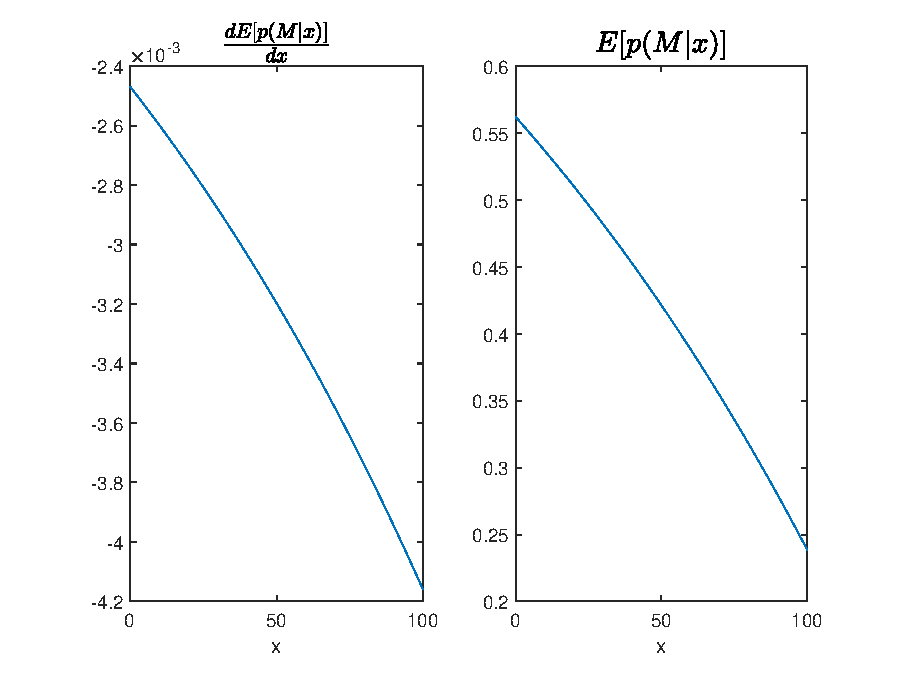
\includegraphics[width=0.5\textwidth]{p_x & dp_x.eps}
    \caption{给定参数下的$E[p(M|x)]$与$\frac{d E[p(M|x)]}{d x}$}
\end{figure}

\par 在同样的参数条件下,给出不同的已有停车位$b$,我们都可以得到停车者的最优停止搜寻位置$x$,可以认为$x_0$是关于$b$的函数。根据前文的$Stop$函数可以发现,在单通道情况下,$Stop$函数值始终大于0,因此只需调整参数$b$直到其与$E_{net}$的零点重合,即可得到单通道结构下停车者的均衡停止搜索位置。根据前文提到的,$\frac{\partial E_{net}}{\partial b}$为负数,因此$E_{net}$的零点会随着$b$的增大而减小。因此我们可以通过调整$b$的值来找到$E_{net}$的零点$x_0$。下图为不同$b$值对应的$x_0$的图像:

\begin{figure}[H]
    \centering
    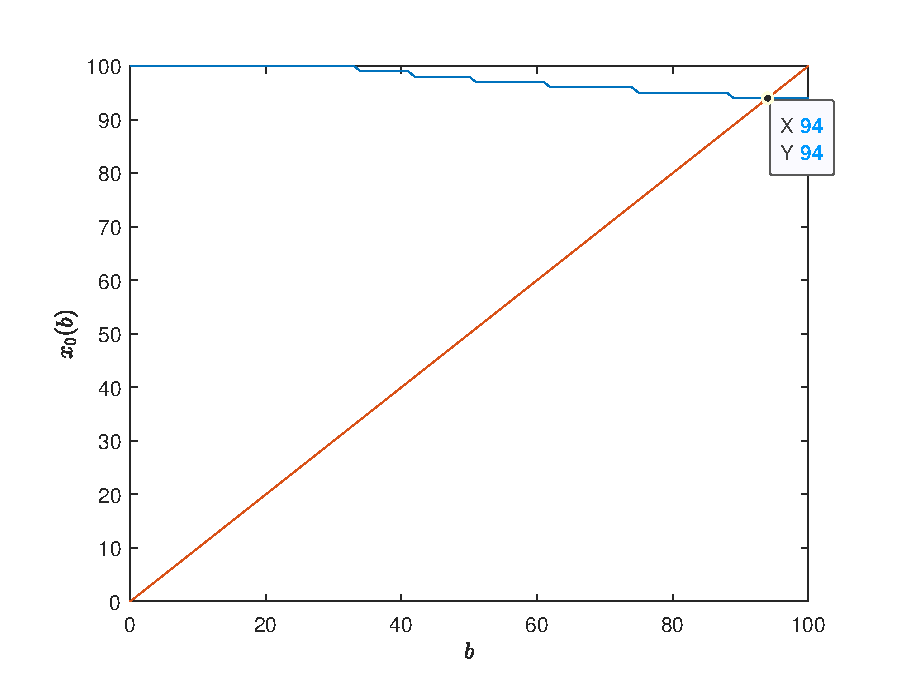
\includegraphics[width=0.5\textwidth]{single_entrance_b_x.eps}
    \caption{不同$b$值与其对应的最优停止搜索点}
    \label{fig:2}
\end{figure}

\begin{figure}[H]
    \centering
    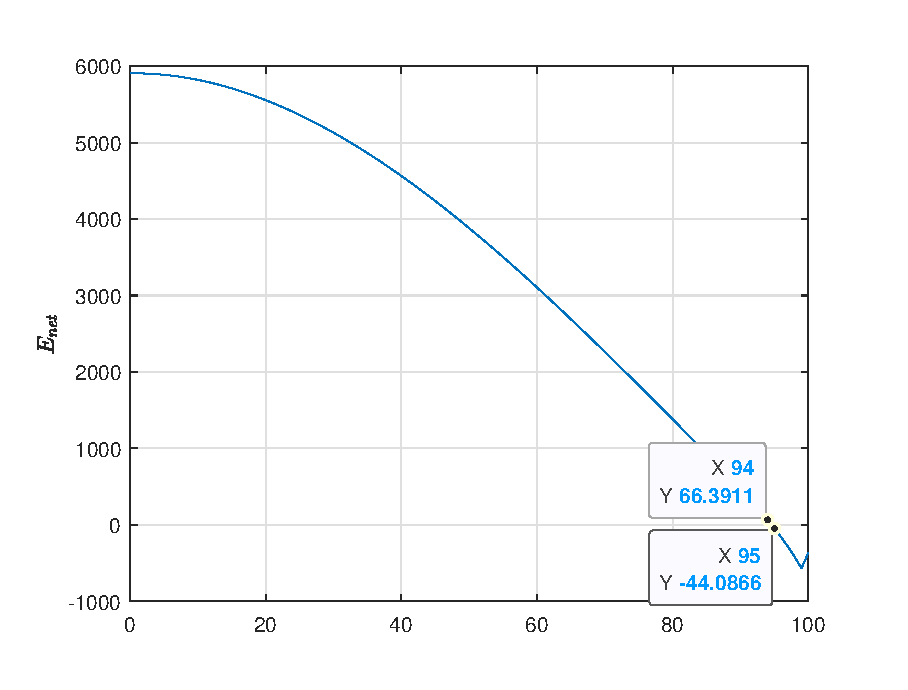
\includegraphics[width=0.5\textwidth]{single_entrance.eps}
    \caption{给定参数下的单向通道情景}
    \label{fig:3}
\end{figure}

\par 根据图\ref{fig:2}可以发现在$b=94$时,最优停止搜索点即为$94$,因此这一点便为给定参数下的单向通道情景的“均衡停止搜索点”,即$\bar{b}~s.t.x_0(\bar{b})=\bar{b}$。在此基础上,通过求目的地位置$e$与均衡停止搜索点$\bar{b}$的差,则可以得到均衡停止搜索点的偏离距离$d(e)$(单通道下$e=100$),用以衡量这一结构下停车场的整体效率。
\par 不仅如此,还可以注意到最优停止搜索点在$b\geq 34$时开始偏离目的地,且偏离距离并随着$b$的增大而增加。这符合现实情况中大量自行车聚集在靠近目的地但仍离目的地有一段距离的地方。图\ref{fig:3}就是均衡参数条件下,即$b=x_0=94$时,$x$与$E_{net}$的图像

\par 值得注意的是,单通道结构下这一结论十分稳健,即使我们适度调整$E_{net}$中参数和子函数的形式,仍然能得到类似的结果。只需要保证以下几点:1. $u'(x)$显著大于$c'(x)$;2. $p(x)$的概率密度函数为平滑的单调递减函数。而这两点几乎可以覆盖全部现实情况。

\par 因此,下面这四次模拟在固定$u'(x)=5$的基础上,调整了$c'(x)$和$p(x)$的形式。其中当$p(x)$为凹函数时,其函数形式为前文中的模型一致,即为$\sum_{m=0}^{N}f_M(m)\cdot [1-(1-p_0+p_1x)^{m-1}]$;当$p(x)$为凸函数时,其形式为$p_x=\frac{11.25}{x+12.5}$\footnote{此处配置这两个系数用以决定$p(x)$的值域,为$[0.1,0.9]$。}。可以发现,即使$c'(x)$和$p(x)$的形式发生了较大变化,最优停车位置$x$仍然保持在靠近入口但不是最靠近的地方,说明单通道结构下这一结论是较为稳健的。

\begin{figure}[H]
    \centering
    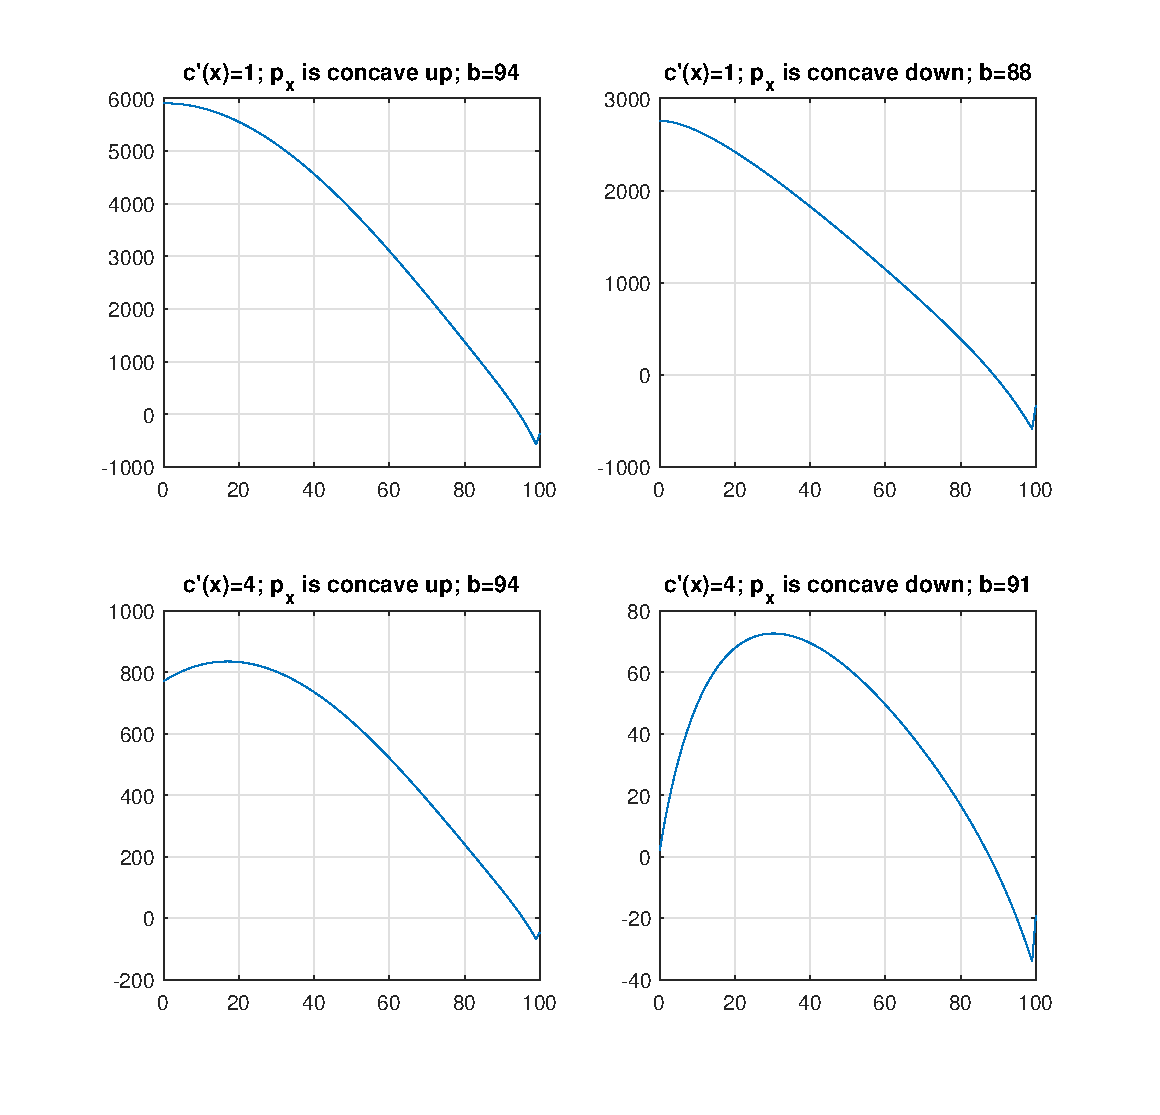
\includegraphics[width=0.5\textwidth]{single_entrance_robust.eps}
    \caption{单入口情景的稳健性检验}    
\end{figure}

\subsection{对称双向通道情景}

\par 类似地,我们可以推广到双向通道情景。在双向通道情景下,停车者可以从任意一个方向进入停车场。这里假设目的地位于整个停车场的正中央,即停车位是关于目的地对称的。因此原模型中与停车场结构相关的函数便需要进行调整。根据$p_x$的形式可以发现其主要受到函数$f_M$和$p_dx$影响,而$f_M$只描述总空车位数量,因此我们只需要调整$p_dx$的形式即可。这里在函数分段后直接加入线性系数$\alpha$保证$p_dx$在定义域内的累加总和为1,即:
$$p_dx = \begin{cases}
    \alpha(p_0-p_1x), & x\leq \frac{N}{2}\\
    \alpha[p_0-p_1(N-x)], & x>\frac{N}{2}
\end{cases}$$
其中$\alpha = \frac{1}{2\cdot\sum_{x=0}^{\frac{N}{2}}(p_0-p_1x)}$。\\
在与单通道情景参数相同时,新的$p_x$图像如下:

\begin{figure}[H]
    \centering
    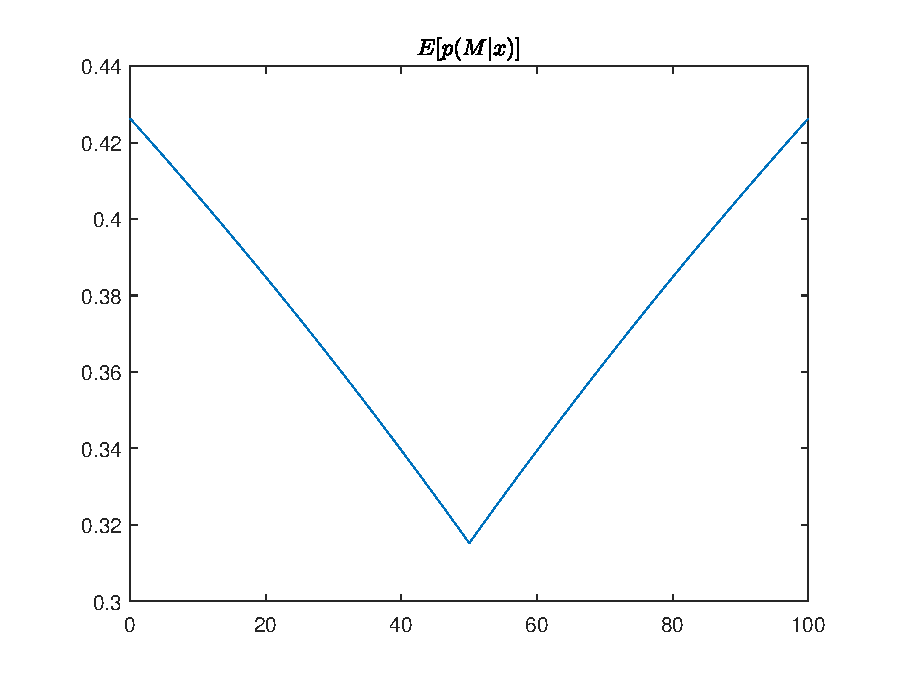
\includegraphics[width=0.5\textwidth]{double_entrance_p_x.eps}
    \caption{双向通道情景下的$p(x)$}
\end{figure}

\par 另一处需要调整的是$u(x)$的形式,由于目的地位于停车场中央的结构天然地优于单向停车场的结构(到达与目的地同样距离的位置,单向通道需要付出更高的成本)。因此出于可比性的考虑,既要保证双向通道与单通道模型在距离目的地相同的位置提供的效用相同;又要保证整个停车场提供的总效用相同。然而这两个条件并不能被同时满足,所以出于谨慎考虑,本文将给出在分别满足这两个前提下的模型均衡解。

\begin{figure}[H]
    \centering
    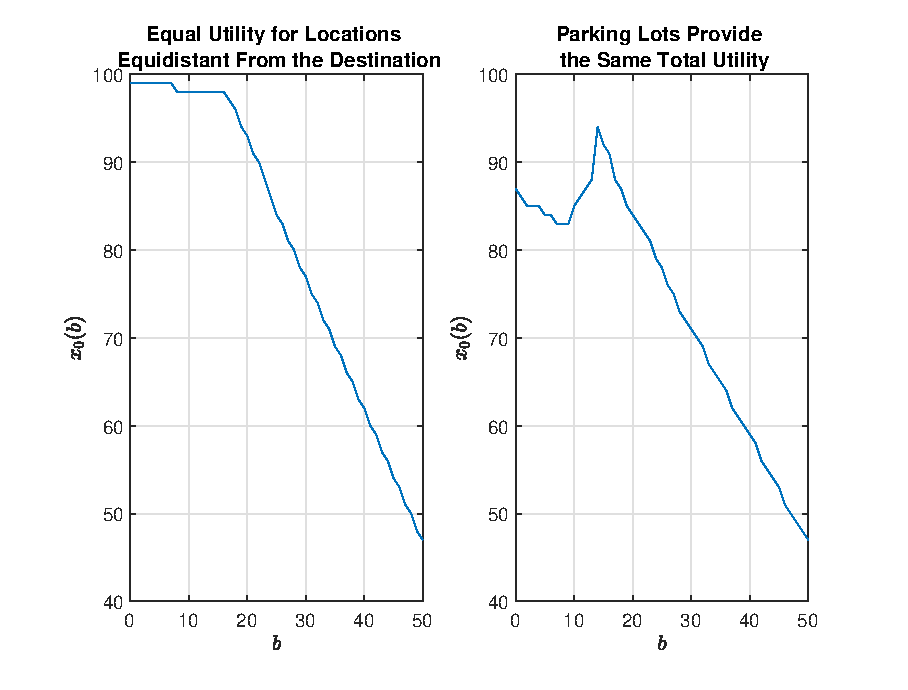
\includegraphics[width=0.5\textwidth]{double_entrance.eps}
    \caption{对称双向通道的两种情况}
    \label{fig:6}
\end{figure}

\par 由于停车场拥有对称结构,因此从任何一侧进入停车场均是等价的。从图\ref{fig:6}可以看到,双向通道情况下,不论是哪种$u(x)$函数,只有在$b$极为接近目的地时(左图中为$b\geq 49$,右图为$b\geq 48$)才会出现搜索范围无法覆盖目的地的情况。因此,不同于单通道结构停车场中的停车者,双向通道的停车者在绝大多数情况下会更倾向于扩大搜索范围,并足够覆盖到目的地。这一点也符合现实中双向通道停车场中央的车位总是很快被占满的情况。

\begin{figure}[H]
    \centering
    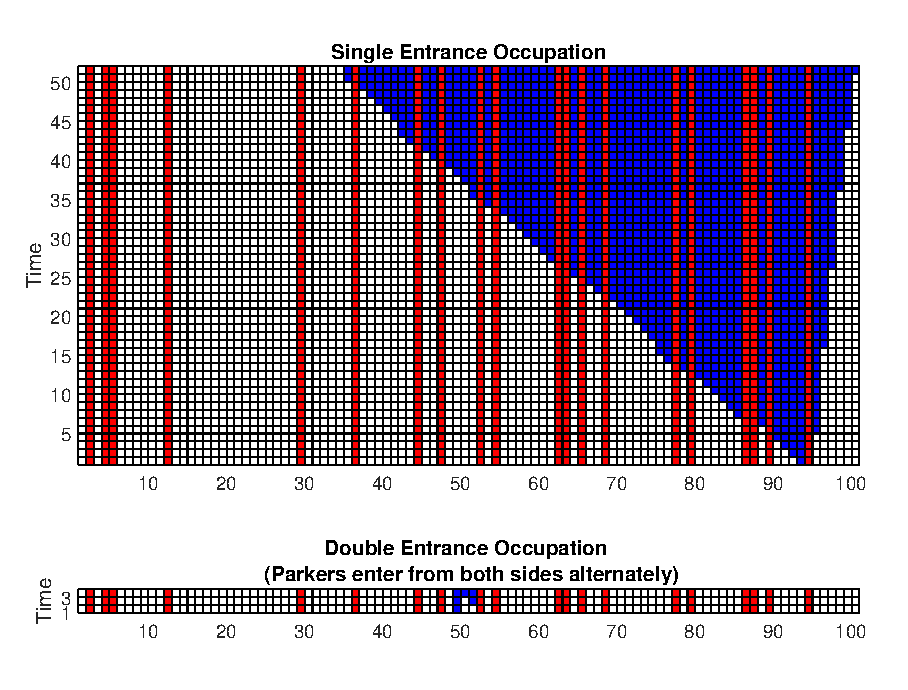
\includegraphics[width=0.5\textwidth]{occupation.eps}
    \caption{两种结构停车场的模拟停车位置}
    \label{fig:7}
\end{figure}

\par 图\ref{fig:7}是模拟停车者在决策函数指导下,分别在双向通道和单通道下的停车位置,不同格子表示特定时刻该位置被占情况,这里假定每一单位时间只有一名停车者进入。其中两种结构停车场中默认被占车位均是随机生成且相同的(图中红色的格子)。这里由于双向通道是对称的,因此新进入的停车者由两侧交替进入停车场(所停位置为图中蓝色格子)。可以发现双向通道情景下目的地处的车位只需在短短3个单位时间内被占用,远快于单通道。其它优质车位也是如此。

\subsection{非对称双向通道情景}
\par 在非对称双向通道情景下,由于停车场的两个进入口距离目的地距离不同,所以停车者可能在了解停车场结构的情况下更加偏好从某一个进入口进入,导致入口距离目的地更近的一侧每个位置有空车位的概率下降。然而这种概率的变化又会反过来影响停车者的选择,即更少的停车者愿意从这一侧进入,从而又使得这一侧的车位利用率上升。
\par 上述的这种负反馈调节必然会达到一个均衡状态,但是出于简化问题的考虑,下面假设停车者对入口的选择是随机的,即距离目的地相同位置有空车位的概率相同。

\begin{figure}[H]
    \centering
    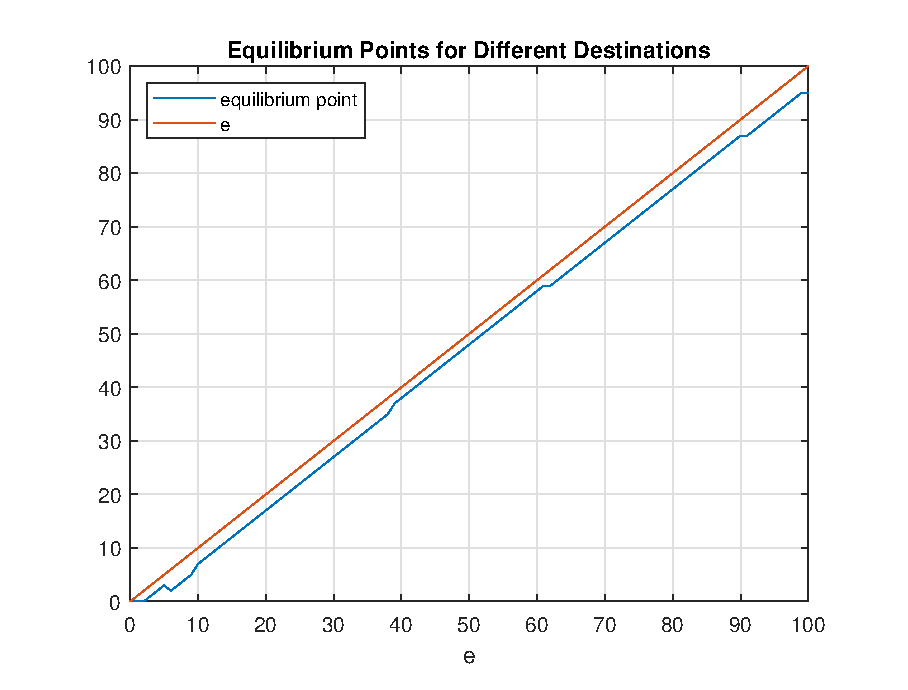
\includegraphics[width=0.5\textwidth]{asymmetric_eq_to_e.eps}
    \caption{不同目的地位置对应的均衡停止搜索点}
    \label{fig:8}
\end{figure}

\par 根据模拟计算,图\ref{fig:8}显示了从任意一侧进入停车场后,目的地$e$位于不同位置时,停车者的均衡停止搜寻点$\bar{b}(e)$的位置。在对$e$和$\bar{b}(e)$求差后,可以得到不同目的地对应的偏离距离$d(e)$。但是由于停车场两侧均可进入,所以双通道下总偏离距离应当为$D(e)=d(e)+d(N-e)$,其与$d$的关系由图\ref{fig:9}所示。
\par 根据图\ref{fig:9}可以观察到,在目的地由两侧向中央移动的过程中,总偏移距离经历了一个先增加后减小的过程,而在中央位置附近($e\in[39,61]$),总偏移距离达到了最小值($min\{D(e)\}=4$)。



\begin{figure}[H]
    \centering
    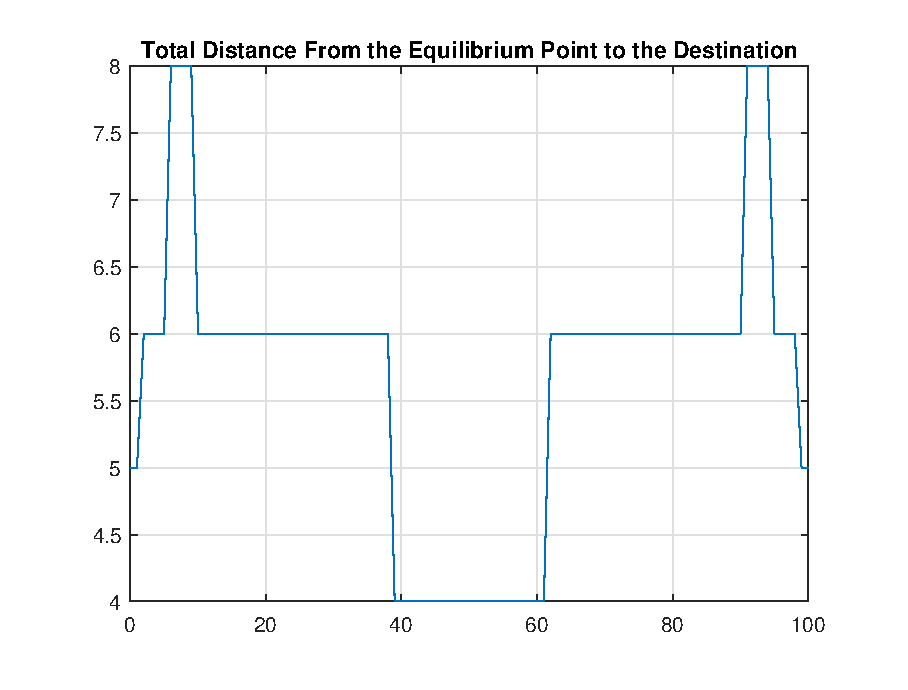
\includegraphics[width=0.5\textwidth]{asymmetric_dstnc_to_e.eps}
    \caption{不同目的地位置对应的总偏离距离}
    \label{fig:9}
\end{figure}


\section{总结与展望}
\subsection{结论}
\par 根据本文的建模和对比可以得出以下结论:当停车场结构为对称的双向通道时,停车场优质车位的利用率要高于单向通道;而当双向通道不对称时,如果目的地处于靠近中心的位置,这一结论仍然成立。这说明在资源的整体利用效率上,双向通道结构在普遍情况下要优于单向通道。
\par 停车场问题本质上是一个搜寻匹配问题,因此上面的结论在其他搜寻匹配问题中也同样适用。即当一个市场只有一个进入口且搜寻成本与资源质量成正比时,市场中最为优质的资源很可能因为搜寻成本的原因而无人问津;而如果市场结构为双向通道,那么这一问题在一定程度上会得到缓解。以人才市场为例,岗位越优质,其对应聘者前期准备和投入的要求就越高。此时由于应聘者竞聘新岗位时可能对已有职务产生不利影响,甚至丢掉现有的工作(例如原单位领导发现此人有跳槽意向),因此应聘者可能会选择放弃前往更优质的岗位的机会。此时招募人才的企业为了吸引更多优质人才,可以在提供目标岗位的同时提供略低于目标岗位的岗位,用作竞聘目标岗位失败的但较优质人才的备选岗位。这种设计相当于将市场结构由单向通道变为双向通道,从而提高了整体资源利用效率。

\subsection{补充与完善}
\par 为了使得模型更加贴近现实,我们可以考虑加入视野以及在$p(x)$函数中实时更新停车者对停车场总共可用车位$M$数量的猜测。前者本质上是为停车者提供若干个零成本向前搜寻的机会;而后者则可使用已找到的空车位的数量与已经查看过的所有车位数进行估计。这两个因素的加入将使得停车者的决策更加复杂,但也更加贴近现实。
\par 尽管如此,这并不影响本文的结论,因为前者相当于在成本函数$c(x)$中减去一个小的常数项。后者只在给定的停车场空间中模拟停车者的决策过程时可以使用,即只会影响图\ref{fig:7}的模拟结果;而在理论求解均衡最优位置$\bar{b}(e)$时,仍需采取本文中使用LOTUS法则求期望的方法消去$p(x)$函数中的$M$。



\bibliographystyle{plainnat}
\bibliography{ref.bib} 

\end{document}